\documentclass[border=8pt,tikz]{standalone}
\usepackage{amsmath,amssymb}
\usepackage{tikz}
\usetikzlibrary{arrows.meta,calc,decorations.pathreplacing,patterns,shapes.geometric,positioning,shadings,plotmarks}

\begin{document}
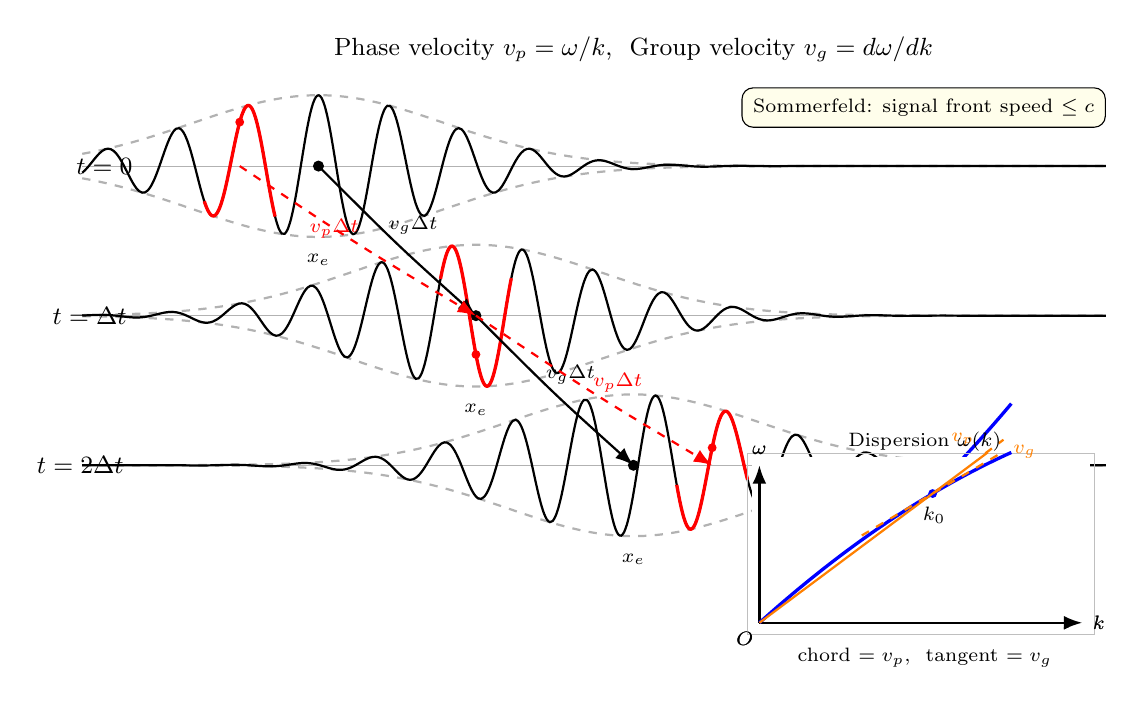
\begin{tikzpicture}[>=Latex,font=\small]

% ============================================================
% Top title
% ============================================================
\node[anchor=south,font=\small] at (7.0,5.2) {Phase velocity $v_p=\omega/k$, \ Group velocity $v_g=d\omega/dk$};

% ============================================================
% MAIN FIGURE: three snapshots of a Gaussian wave packet
% Horizontal extent: x from 0 to 13
% Three baselines: y = 4.0 (t=0), y = 2.3 (t=dt), y = 0.6 (t=2 dt)
% ============================================================

% --- Envelope parameters ---
% Envelope centers:
%   x_e(0)    = 3.0
%   x_e(dt)   = 5.0    (group speed v_g*dt = 2.0)
%   x_e(2dt)  = 7.0
% Tracked peak:
%   x_p(0)    = 2.0    (inside left shoulder of envelope)
%   x_p(dt)   = 5.0    (at envelope center)
%   x_p(2dt)  = 8.0    (past envelope right shoulder)
%   => peak speed v_p*dt = 3.0  vs  v_g*dt = 2.0   (ratio 3:2)
% Envelope sigma:
%   sigma = 1.6 (wide enough to contain oscillation visibly)
% Carrier:
%   k = 7   (about 10 oscillations across envelope FWHM ~ 3.8)

% ---------- snapshot t=0 ----------
\begin{scope}[yshift=4cm]
  % axis baseline
  \draw[gray!60,very thin] (0,0) -- (13,0);
  % envelope outline (gaussian, dashed grey)
  \draw[gray!60,dashed,thick,domain=0:13,samples=160,smooth]
      plot (\x,{0.9*exp(-((\x-3.0)^2)/(2*1.6*1.6))});
  \draw[gray!60,dashed,thick,domain=0:13,samples=160,smooth]
      plot (\x,{-0.9*exp(-((\x-3.0)^2)/(2*1.6*1.6))});
  % modulated carrier (black)
  \draw[black,thick,domain=0:13,samples=360,smooth]
      plot (\x,{0.9*exp(-((\x-3.0)^2)/(2*1.6*1.6))*cos(7*(\x-3.0) r)});
  % envelope center dot
  \fill[black] (3.0,0) circle (2pt);
  \node[below,font=\scriptsize] at (3.0,-1.0) {$x_e$};
  % tracked peak (red) at x = 2.0, around this peak we draw a red arc of the carrier
  \draw[red,very thick,domain=1.55:2.45,samples=80,smooth]
      plot (\x,{0.9*exp(-((\x-3.0)^2)/(2*1.6*1.6))*cos(7*(\x-3.0) r)});
  \fill[red] (2.0,{0.9*exp(-((2.0-3.0)^2)/(2*1.6*1.6))*cos(7*(2.0-3.0) r)}) circle (1.6pt);
  % time label
  \node[anchor=west,font=\small] at (-0.2,0) {$t=0$};
\end{scope}

% ---------- snapshot t=dt ----------
\begin{scope}[yshift=2.1cm]
  \draw[gray!60,very thin] (0,0) -- (13,0);
  \draw[gray!60,dashed,thick,domain=0:13,samples=160,smooth]
      plot (\x,{0.9*exp(-((\x-5.0)^2)/(2*1.6*1.6))});
  \draw[gray!60,dashed,thick,domain=0:13,samples=160,smooth]
      plot (\x,{-0.9*exp(-((\x-5.0)^2)/(2*1.6*1.6))});
  \draw[black,thick,domain=0:13,samples=360,smooth]
      plot (\x,{0.9*exp(-((\x-5.0)^2)/(2*1.6*1.6))*cos(7*(\x-2.0) r)});
  \fill[black] (5.0,0) circle (2pt);
  \node[below,font=\scriptsize] at (5.0,-1.0) {$x_e$};
  % tracked peak now at x = 5.0 (center)
  \draw[red,very thick,domain=4.55:5.45,samples=80,smooth]
      plot (\x,{0.9*exp(-((\x-5.0)^2)/(2*1.6*1.6))*cos(7*(\x-2.0) r)});
  \fill[red] (5.0,{0.9*exp(-((5.0-5.0)^2)/(2*1.6*1.6))*cos(7*(5.0-2.0) r)}) circle (1.6pt);
  \node[anchor=west,font=\small] at (-0.5,0) {$t=\Delta t$};
\end{scope}

% ---------- snapshot t=2 dt ----------
\begin{scope}[yshift=0.2cm]
  \draw[gray!60,very thin] (0,0) -- (13,0);
  \draw[gray!60,dashed,thick,domain=0:13,samples=160,smooth]
      plot (\x,{0.9*exp(-((\x-7.0)^2)/(2*1.6*1.6))});
  \draw[gray!60,dashed,thick,domain=0:13,samples=160,smooth]
      plot (\x,{-0.9*exp(-((\x-7.0)^2)/(2*1.6*1.6))});
  \draw[black,thick,domain=0:13,samples=360,smooth]
      plot (\x,{0.9*exp(-((\x-7.0)^2)/(2*1.6*1.6))*cos(7*(\x-1.0) r)});
  \fill[black] (7.0,0) circle (2pt);
  \node[below,font=\scriptsize] at (7.0,-1.0) {$x_e$};
  % tracked peak at x = 8.0 (past right shoulder)
  \draw[red,very thick,domain=7.55:8.45,samples=80,smooth]
      plot (\x,{0.9*exp(-((\x-7.0)^2)/(2*1.6*1.6))*cos(7*(\x-1.0) r)});
  \fill[red] (8.0,{0.9*exp(-((8.0-7.0)^2)/(2*1.6*1.6))*cos(7*(8.0-1.0) r)}) circle (1.6pt);
  \node[anchor=west,font=\small] at (-0.7,0) {$t=2\Delta t$};
\end{scope}

% ---------- Arrows showing envelope center drift and tracked peak drift ----------
% envelope center trajectory (black dashed arrow between snapshots)
\draw[black,thick,->] (3.0,4.0) .. controls (4.0,3.0) and (4.0,3.0) .. (5.0,2.1);
\draw[black,thick,->] (5.0,2.1) .. controls (6.0,1.1) and (6.0,1.1) .. (7.0,0.2);
\node[black,font=\scriptsize] at (4.2,3.25) {$v_g\Delta t$};
\node[black,font=\scriptsize] at (6.2,1.35) {$v_g\Delta t$};

% tracked peak trajectory (red dashed arrow)
\draw[red,thick,->,dashed] (2.0,4.0) .. controls (3.5,3.0) and (3.5,3.0) .. (5.0,2.1);
\draw[red,thick,->,dashed] (5.0,2.1) .. controls (6.5,1.1) and (6.5,1.1) .. (8.0,0.2);
\node[red,font=\scriptsize] at (3.2,3.2) {$v_p\Delta t$};
\node[red,font=\scriptsize] at (6.8,1.25) {$v_p\Delta t$};

% ---------- legend / annotations box ----------
\node[draw,rounded corners,fill=yellow!8,inner sep=4pt,font=\scriptsize,align=left,anchor=north east]
  at (13.0,5.0)
  {Sommerfeld: signal front speed $\le c$};

% ============================================================
% INSET (bottom right): omega(k) dispersion curve
% Inset frame: x in [8.5,13], y in [-3.2, -0.2]
% ============================================================
\begin{scope}[shift={(10.7,-1.7)}]
  % axes
  \draw[->,thick] (-2.1,-0.1) -- (2.0,-0.1) node[right,font=\scriptsize] {$k$};
  \draw[->,thick] (-2.1,-0.1) -- (-2.1,1.9) node[above,font=\scriptsize] {$\omega$};
  % origin label
  \node[font=\scriptsize,anchor=north east] at (-2.05,-0.1) {$O$};

  % dispersion curve: slightly concave-up (normal dispersion: chord slope > tangent slope)
  % we'll use omega(k) = 0.55*k + 0.10*k*k  shifted so it starts at origin region
  % plotted with k' = \x from 0 to 3.2, shifting x into local coords: x_local = \x - 2.0
  \draw[blue,very thick,domain=0:3.2,samples=80,smooth]
      plot ({\x-2.1},{0.55*\x + 0.10*\x*\x - 0.1});

  % chosen point k_0 at \x = 2.0 (local x = -0.1)
  % omega(k_0) = 0.55*2.0 + 0.10*4.0 - 0.1 = 1.1 + 0.4 - 0.1 = 1.4
  \pgfmathsetmacro{\xz}{2.0}
  \pgfmathsetmacro{\oz}{0.55*\xz + 0.10*\xz*\xz - 0.1}
  \pgfmathsetmacro{\xl}{\xz - 2.1}
  \fill[blue] (\xl,\oz) circle (1.4pt);
  \node[font=\scriptsize,anchor=north west] at (\xl+0.05,\oz-0.02) {$k_0$};

  % chord from origin (-2.1,-0.1) to (xl, oz)  — slope = omega/k = v_p
  \draw[orange,thick,dashed] (-2.1,-0.1) -- ($(\xl,\oz)+0.55*({\xl-(-2.1)},{\oz-(-0.1)})$);
  \node[orange,font=\scriptsize,anchor=south] at (-0.9,0.5) {$v_p=\omega/k$};

  % tangent line at k_0: slope = 0.55 + 0.20*k_0 = 0.55 + 0.40 = 0.95  (but chord slope = 1.5/2.0 = 0.75 ... we need tangent < chord for normal)
  % Actually with a CONVEX-UP curve (concave up), tangent > chord. We want tangent < chord (v_g < v_p).
  % So we should use a CONCAVE curve (second derivative negative): omega(k) = 0.9*k - 0.08*k*k
  % Redo: remove previous curve and redraw with concave form.
\end{scope}

% Clear and redraw inset with correct (concave) curve so that tangent slope < chord slope.
\begin{scope}[shift={(10.7,-1.7)}]
  \fill[white] (-2.2,-0.15) rectangle (2.1,2.0);
  % frame box for the inset
  \draw[gray!50,thin] (-2.25,-0.25) rectangle (2.15,2.05);

  % axes
  \draw[->,thick] (-2.1,-0.1) -- (2.0,-0.1) node[right,font=\scriptsize] {$k$};
  \draw[->,thick] (-2.1,-0.1) -- (-2.1,1.9) node[above,font=\scriptsize] {$\omega$};
  \node[font=\scriptsize,anchor=north east] at (-2.05,-0.1) {$O$};

  % concave curve: omega(k) = 0.9*k - 0.07*k*k  (for k from 0 to 3.2)
  % k=0 : 0 ; k=3.2 : 2.88 - 0.717 = 2.16  -> close to top
  \draw[blue,very thick,domain=0:3.2,samples=80,smooth]
      plot ({\x-2.1},{0.9*\x - 0.07*\x*\x - 0.1});

  % chosen point k_0 = 2.2
  \pgfmathsetmacro{\xz}{2.2}
  \pgfmathsetmacro{\oz}{0.9*\xz - 0.07*\xz*\xz - 0.1}
  \pgfmathsetmacro{\xl}{\xz - 2.1}
  \fill[blue] (\xl,\oz) circle (1.6pt);
  \node[font=\scriptsize,anchor=north] at (\xl+0.02,\oz-0.05) {$k_0$};

  % --- chord: from origin (-2.1, -0.1) to (xl, oz); chord slope in local coords = (oz+0.1)/(xl+2.1)
  % extend chord a bit beyond the point:
  \pgfmathsetmacro{\chordEndX}{\xl+0.7}
  \pgfmathsetmacro{\chordSlope}{(\oz+0.1)/(\xl+2.1)}
  \pgfmathsetmacro{\chordEndY}{-0.1 + \chordSlope*(\chordEndX+2.1)}
  \draw[orange,thick] (-2.1,-0.1) -- (\chordEndX,\chordEndY);
  \node[orange,font=\scriptsize,anchor=south east] at (\chordEndX-0.05,\chordEndY-0.05) {$v_p$};

  % --- tangent at k_0: slope = 0.9 - 0.14*k_0 = 0.9 - 0.308 = 0.592 (in "natural" coords)
  \pgfmathsetmacro{\tanSlope}{0.9 - 0.14*\xz}
  % tangent from (xl,oz) extending both directions
  \pgfmathsetmacro{\tanStartX}{\xl-0.9}
  \pgfmathsetmacro{\tanStartY}{\oz - \tanSlope*0.9}
  \pgfmathsetmacro{\tanEndX}{\xl+0.9}
  \pgfmathsetmacro{\tanEndY}{\oz + \tanSlope*0.9}
  \draw[orange,thick,dashed] (\tanStartX,\tanStartY) -- (\tanEndX,\tanEndY);
  \node[orange,font=\scriptsize,anchor=west] at (\tanEndX,\tanEndY) {$v_g$};

  % inset title / caption
  \node[font=\scriptsize,anchor=south] at (-0.0,1.95) {Dispersion $\omega(k)$};
  \node[font=\scriptsize,anchor=north,align=center] at (0.0,-0.3) {chord $=v_p$, \ tangent $=v_g$};
\end{scope}

\end{tikzpicture}
\end{document}
